\section{Revisão da Literatura}
\qquad A disciplina \textcolor{blue}{Comportamento Organizacional} é uma ciência aplicada ao comportamento que é retirada de contribuições de disciplinas que estudam o comportamento, especificamente da psicologia e psicologia social, sociologia e antropologia.
As contribuições da psicologia são concentrada no individuo ou analise a nível micro, enquanto as outras disciplinas contribuíram para perceber a nível macro conceitos como procedimentos de grupo e organização.\cite{book_2}
\emptyline
Quadro das Contribuições para o estudo desta disciplina:
\begin{figure}[H]
\centering
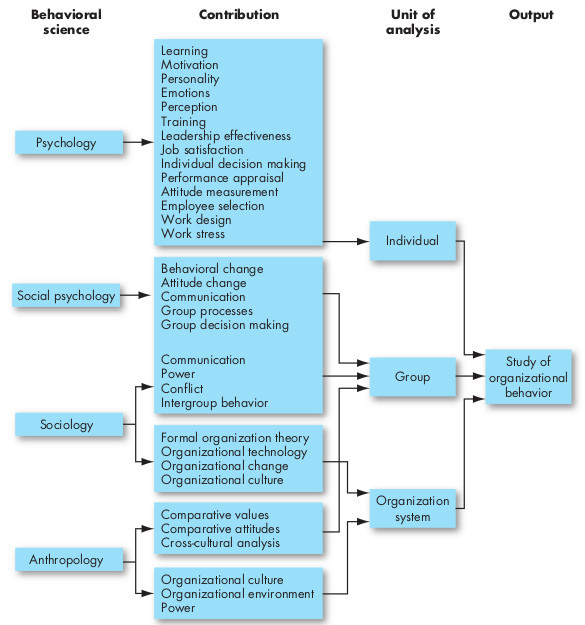
\includegraphics[scale=0.52]{./image/OB/OB_contributions.jpg}
\caption{Contribuições para OB \cite{book_2}}
\end{figure}
Este relatório esta focado no estudo da \textcolor{blue}{\textbf{Cultura Organizacional}}, portanto vou começar por definir o que é uma organização e seus objetivos.
\emptyline
%%%%%%%%%%%%%%%%%%%%%%%%%%%%%
Uma organização é um grupo estruturado de pessoas, um grupo onde cada pessoa é responsável por tarefas bem definidas e onde existe um sistema de articulação entre elas, que desenvolve um conjunto de atividades visando a definição e prossecução de objetivos comuns (de forma continuada no tempo). O objetivo das organizações é para criar valor para os seus clientes/utentes, para os detentores do seu capital, para os seus colaboradores, para os seus fornecedores e para a sociedade em geral.\cite{book_10}
%%%%%%%%%%%%%%%%%%%%%%%%%%%%%%%%%%%%%%%%%%%%%%%%%%%%%%%%%%%%%%%%%%%%%%%%%%%%%%%%%%%%%%%%%%%%%%%%%%%%%%%%%%%%%%%
\newpage
Todas as organizações estão inseridas num contexto Cultural que pertence a um País ou Região e pelo modelo criado por \textit{Geer Hofstede}, Portugal tem esta distribuição nas suas dimensões:
\begin{figure}[H]
\begin{minipage}{0.3\textwidth}
\flushleft
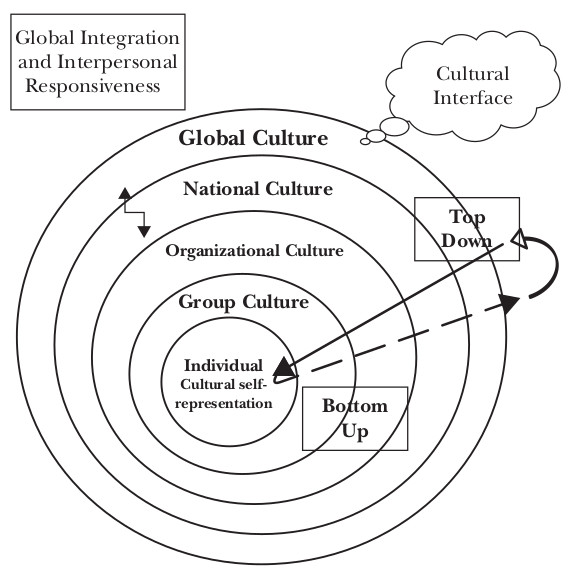
\includegraphics[scale=0.30]{./image/OB/OB_MUltilevelmodelCulture.jpg}
\end{minipage}
\hspace{.1cm}
\begin{minipage}{0.4\textwidth}
\flushleft
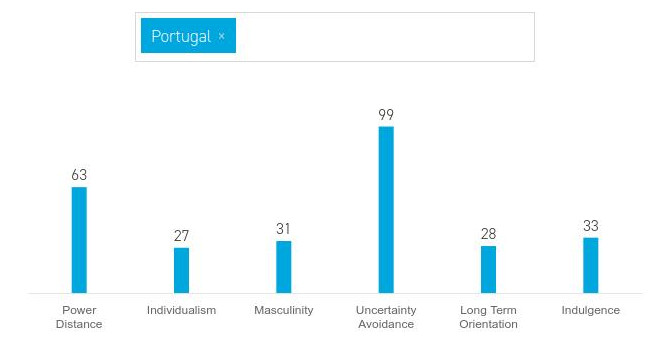
\includegraphics[scale=0.45]{./image/OB/Hofstede_pt.jpg}
\end{minipage}
\caption{Modelo de Multi-níveis \cite{book_11} da cultura e Modelo Hofstede, Portugal}
\end{figure}
Website:\\
\textit{\textcolor{green}{https://hi.hofstede-insights.com/national-culture}}
\emptyline
%%%%%%%%%%%%%%%%%%%%%%%%%%%%
Ambos a Cultura da Organização e o Comportamento da Liderança foram identificados como determinantes criticos para a eficácia da organização, que se deve adaptar ao contexto transacional e externo à organização. A Cultura Organizacional é um conjunto de valores, crenças e suposições partilhadas pelos membros de uma organização que a distingue das outras organizações, por exemplo, rituais e cerimonias, a historia da organização, sua estrutura e seus princípios.\cite{book_9}
\emptyline
%%%%%%%%%%%%%%%%%%%%%%%%%%%%%
A forma das organizações se identificarem e destacarem a sua cultura no mercado é expondo a sua \textcolor{blue}{Missão}, \textcolor{blue}{Visão} e seus \textcolor{blue}{Valores}.
\emptyline
%%%%%%%%%%%%%%%%%%%%%%%%%%%%%
A \textcolor{blue}{missão} é os objetivos na qual a organização pretende atingir, a \textcolor{blue}{visão} aonde pretendem chegar (futuro) e seus \textcolor{blue}{valores}, que são suas crenças e princípios na qual defendem, e mantêm a organização unida. Como vimos anteriormente pelo estudo de \textit{Geer Hofsteed} os valores são dependente das culturas.
\emptyline
%%%%%%%%%%%%%%%%%%%%%%%%%%%%%%
As Organizações podem ter diferentes características, e o \textcolor{blue}{\textbf{Modelo de Ogbonna \& Harris}}, carateriza a cultura das organizações em \textcolor{orange}{quatro} tipos, que pode ser análoga a outros modelos tais como o de \textbf{Handy} e \textbf{Cameron \& Quin}.
\begin{figure}[H]
\flushleft
\captionsetup{justification=raggedright,singlelinecheck=false}
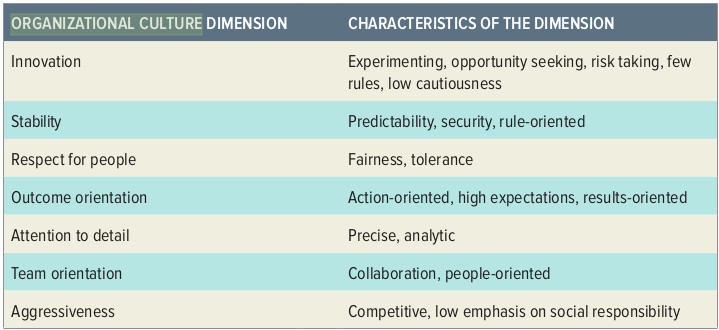
\includegraphics[scale=0.4]{./image/OB/OC_Dimensions.jpg}
\caption{Dimensões da Cultura Organizacional \cite{book_4}}
\end{figure}
A cultura de uma organização pode ser descrita como a perceção em que todos seus membros tem em comum acerca da organização, normalmente a maioria de grandes organizações podem ter uma cultura dominante com varias subculturas, sua cultura dominante reflect seus valores de raiz, e subculturas podem ter os valores de raiz mais alguns outros valores únicos dos seus membros de um dado departamento. \\
A cultura organizacional dominante pode ser medida em termos da quantidade em que seus membros estão alinhados com os valores de raiz. \\
As organizações devem criar uma cultura organizacional em que proporciona um \textcolor{blue}{clima} favorável para seus membros de forma a poderem ter um desempenho positivo, caso contrario pode ter o efeito contrario. A cultura organizacional é criada pelos fundadores da organização, com a responsabilidade de a sustentar e cuidar, mantendo seus valores éticos e de moralidade intactos para ter uma \textcolor{blue}{cultura positiva}. O papel da \textcolor{blue}{motivação} tem uma influencia importante na sua manutenção, deve promover a recompensa e delegação de poder.\cite{book_4} \cite{book_2}
%%%%%%%%%%%%%%%%%%%%%%%%%%%%%%%%%%%%%%%%%%%%%%%%%%%%%%%%%%%%%%%%%%%%%%%%%%%%%%%%%
